
\section{Información sobre el proyecto}

\subsection{Sector(es)  en el que se desarrolla el proyecto:}


\subsection{Título:                                        }
\begin{instrucciones}
  El sector puede ser alguno de los propuestos en la convocatoria
  (agricultura, energía, agua, biodiversidad, desarrollo tecnológico e
  innovación) u otros.
\end{instrucciones}
Ciencias Básicas
\subsection{Resumen ejecutivo:                            }
%Máximo 200 palabras.
\subsection{Monto económico total (incluida contrapartida):}
\subsection{Antecedentes:                                  }
Los avances recientes en física de partículas y cosmología han dado
lugar a un entendimiento claro de las tres fronteras a lo largo de la
cual la física de partículas debe avanzar para resolver algunos de los
misterios cruciales de nuestro universo: tales como el origen de la
masa, la naturaleza de la materia oscura y la energía oscura, la
generación de la asimetría materia-antimateria, y la posible
unificación de las fuerzas. Las tres fronteras que se ilustran en la
Figura~\ref{fig:1}, se han identificado como la Frontera de Energía,
la Frontera de Intensidad, y la Frontera Cósmica \cite{fermilab}. Este
proyecto cubrirá las tres frentes y conectará física de partículas y
cosmología. En el proyecto se estudiarán varios modelos teóricos
confrontándolos con los resultados experimentales recientes y haciendo
predicciones para los experimentos en marcha y los que entrarán
próximamente en funcionamiento.

\begin{figure}
  \centering
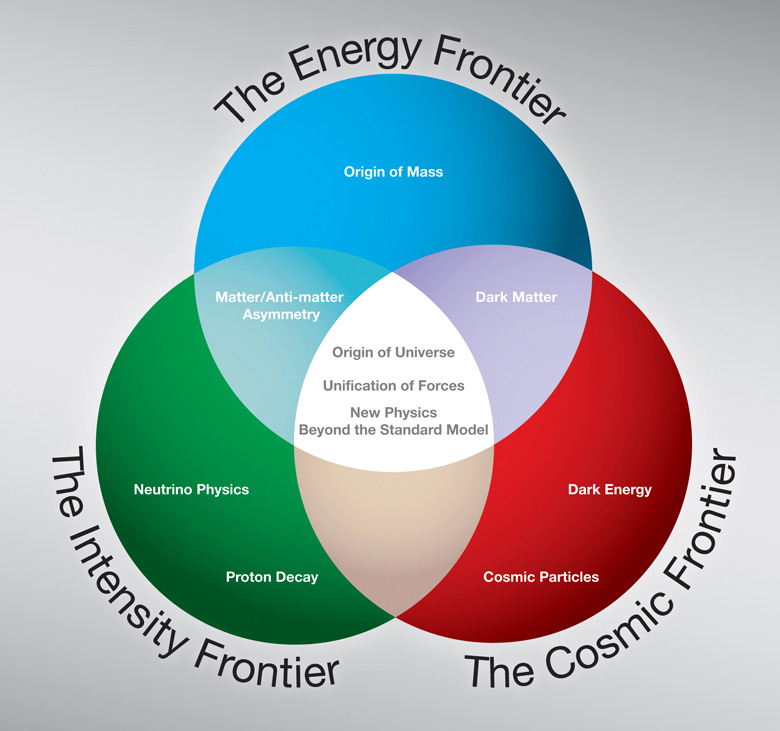
\includegraphics[scale=0.3]{three-frontiers-large}
  \caption{Fronteras de energía. From \cite{fermilab}}
  \label{fig:1}
\end{figure}

Estamos ahora en una época de efervescencia experimental con
detectores de partículas instalados desde las alturas de satélites
artificiales, hasta las profundidades de laboratorios subterráneos a
kilómetros de profundidad. Esto marca una época excitante para la
física de partículas con nuevos datos experimentales disponibles en
las tres fronteras antes mencionadas que de poderse correlacionar
permitirían un entendimiento más profundo de los constituyentes del
Universo.  

La Frontera de Energía, ha alcanzado la escala del Tera, la energía a
la cual se rompe la simetría electrodébil. Para finales del 2012 el
LHC habrá completado su primer ``run'' a una energía de centro de masa
de 7~TeV y habrá acumulado al menos 8/fb de datos. Con esta
luminosidad se podrá vislumbrar una escala de energía que hasta ahora
no había sido explorada. La prioridad es la búsqueda del Higgs del
Modelo Estándar, el cual a la fecha aún no ha sido encontrado. Pero
para comienzos del 2011 se espera obtener la primeras evidencias de su
existencia o excluirlo hasta un rango de masa de unos 600~GeV.

Quizás el resultado experimental más importante en los últimos años de
necesidad de física más allá del modelo estándar (ME) de las partículas
elementales es el descubrimiento de que los neutrinos tienen una masa,
que ha resultado ser pequeña, pero diferente de cero. Esto se ha
deducido a partir de las observaciones de oscilación de neutrinos a
medida que se propagan sobre grandes distancias. Debido a que los
neutrinos interactúan sólo débilmente, los experimentos de neutrinos
requieren de detectores fabricados de materiales masivos y rayos muy
intensos. Los experimentos de neutrinos exploran de ésta manera la
Frontera de Intensidad. Los experimentos en esta frontera se enfocan
ahora en estudios más precisos de oscilaciones de neutrinos así como
en búsqueda de nuevas fuentes de violación de CP, mezcla de sabores de
leptones cargados, decaimientos raros, y en la determinación de la
velocidad de propagación de neutrinos energéticos. Los experimentos
que usan rayos muy intensos a energías inferiores que el LHC pueden
proveer información complementaria a los posibles descubrimientos de
los detectores ATLAS y CMS. Un decaimiento raro que proviene del
intercambio de una partícula de masa alta puede mantener información
sobre las propiedades de el estado intercambiado aunque éste sea
demasiado pesado para ser producido directamente.

La Frontera Cósmica utiliza laboratorios subterraneos, telescopios
basados en tierra y telescopios instalados en satelites para explorar
la componentes oscuras de materia y energía, las huellas de la
inflación y el origen y destino del universo. Las observaciones de la
Frontera Cósmica han alcanzado una precisión mucho mayor de la podría
haber sido imaginada dos decadas antes. Estos han conseguido
determinar detalles del universo primitivo los cuales son cada vez más
consistentes con el ``Modelo Estándar'' de Cosmología basado en la
constante cosmológica y en la materia oscura fría ($\Lambda$CDM), que
dan cuenta del 95\% del contenido energético del Universo. Técnicas
novedosas como lentes gravitacionales, han aportado significativamente
a nuestro conocimiento del pasado cosmológico, en particular en
aumentar la evidencia experimental de que la materia oscura del universo
está compuesta de partículas masivas débilmente interactuantes (WIMPS),
formando halos de materia alrededor de las galaxias. Cómo los 
neutrinos constituyen sólo alrededor del 1\% del contenido energético
del universo, los WIMPS se constituyen en la segunda evidencia
experimental de necesidad de física más allá del ME.  El valor de múltiples
estudios con pruebas diferentes, incluyendo diversos tipos de
partículas, radiación electromagnética sobre un rango muy amplio
incluyendo rayos gamma se hace evidente en el conocimiento detallado
que se ha logrado alcanzar y el que se espera mejorar con los
experimentos que recientemente han entrado en funcionamiento.

El Grupo de Fenomenología de Interacciones Fundamentales de la
Universidad de Antioquia, en colaboración con Grupos emergentes en
otras instituciones la región conformados por egresados de doctorado
de nuestro Grupo nos hemos enfocado en la investigación científica de
aspectos fenomenológicos en estas tres fronteras de la física de altas
energías y la cosmología. Estas investigaciones se han hecho en
colaboración con investigadores internacionales, especialmente con
científicos colombianos trabajando en el exterior. A través de este
proyecto se busca dar continuidad a estos desarrollos a través de
investigaciones de impacto científico en la comunidad científica de
éstas áreas de frontera.

\subsection{Justificación:                                 }
\section{Planteamiento del Problema }
\begin{instrucciones}
  CODI: 

  * ¿Está bien definido el problema que se quiere investigar?:
  Fenomenología de modelos más allá del ME motivados por evidencias
  fenomenológicas del ME.  
  * ¿Es clara su justificación desde el punto de vista académico,
  científico, tecnológico, social, económico y legal? (15).
  científico: contribuir a la correspondiente rama del conocimiento

  COLCI: en este ítem usted deberá describir de forma precisa y completa la
  
  * naturaleza y magnitud del problema de investigación que se quiere
  abordar:
  ** Construir modelos nuevos.
  ** Explorar modelos existentes.
  Formule claramente las preguntas concretas a las cuales se
  quiere responder en el contexto del problema planteado.
\end{instrucciones}
%Tesis
El modelo estándar de las interacciones fundamentales ha sido muy
exitoso durante las últimas décadas para explicar la mayoría de los
resultados experimentales de física de altas energías. Sin embargo,
paralelamente se ha venido acumulando evidencia experimental que
requiere extender el modelo estándar con nuevas partículas. En la
actualidad hay un gran esfuerzo experimental para explorar en detalle
todas estas posibilidades. Estamos ahora en una época de efervescencia
experimental con detectores de partículas instalados desde las alturas
de satelites artificiales, hasta las profundidades de laboratorios
subterráneos a kilometros de profundidad.

El Large Hadron Collider (LHC), en un tunel a 100 metros de profundidad y
con una circunferencia de 27 Km, es el primer acelerador
que puede probar la escala del TeV.  Posee cuatro
detectores, dos de los cuales están especialmente diseñados para
encontrar señales de nueva física. El LHC  ha comenzado a
operar en el 2010, aunque hasta el 2012 lo hará a la mitad de la
energía para la cual fue diseñado. A partir del 2014 aproximandamente, comenzará a funcionar a la energía de diseño de 14\,TeV.

Desde el 2008 varios experimentos sobre rayos cósmicos como ATIC
\cite{:2008zzr} y los satélites PAMELA \cite{Adriani:2008zr} y
Fermi--LAT \cite{Abdo:2009zk}, han venido reportando un exceso en el
flujo de electrones y positrones en rayos cósmicos. Estos resultados
han dado lugar a un sinnúmero de publicaciones tratando de explicar su
origen. Ya se han comenzado a reportar las primeras medidas de rayos
gamma por parte de Fermi--LAT, las cuales pueden ayudar a discernir si
el origen de las anomalías detectadas en electrones y positrones es
debida a fuentes astrofísicas como pulsares cercanos, o a la
aniquilación o el decaimiento de materia oscura. El detector de rayos
cósmicos AMS-02~\cite{ams:2009}, ha sido instalado recientemente en la
estación espacial internacional para medir el espectro de antiprotones
y positrones en un rango de energía mucho más amplio y con una
estadística mucho mejor que PAMELA.

Los experimentos de detección directa de materia oscura instalados en
laboratorios subterráneos como XENON100 \cite{Aprile:2011ts}, han
comenzado a explorar las regiones predichas por algunos de los modelos
más estudiados de materia oscura. Para los próximos años se espera
cubrir todo el espacio de parámetros para materia oscura del modelo
estándar supersimétrico mínimo restringido (Constrained MSSM de sus
siglas en Inglés).  

Finalmente se ha venido acumulando evidencia experimental respecto al último ángulo de mezcla del sector de neutrinos que muestra que dicho ángulo no sólo es diferente de cero sino que puede ser suficientemente grande como para permitir violación de CP en el sector leptónico \cite{valle}. La violación de CP en el sector leptónico es un ingrediente necesario para generar la asimetría de materia-antimateria a través de leptogénesis~\cite{Davidson:2008bu}.


En éste proyecto se explorarán diferentes extensiones del modelo
estándar que explican estos datos y tienen predicciones
concretas para los experimentos presentes y futuros mencionados
anteriormente.

%evidencia 1
La principal evidencia de necesidad de física más allá del modelo
estándar se halla en las medidas de las oscilaciones de neutrinos, que
a través de muchos experimentos diferentes han logrado establecer que
los neutrinos tienen masa y se mezclan entre sí. Si la masa de los
neutrinos es total o parcialmente explicada por métodos radiativos, no
sólo es posible dar cuenta de la pequeñez de sus masas con respecto a
la de los otros fermiones, sino también, hacer predicciones muy
concretas en aceleradores de partículas, como el LHC. Aún en el caso
de modelos tan estudiados de este tipo, como es el caso del modelo
supersimétrico con ruptura bilineal de paridad R, quedan aún muchos
aspectos que explorar.

%evidencia 2
En los últimos tiempos,
\begin{soloproyecto}
sobre todo después de las medidas de
precisión de WMAP, el satelite de la NASA que ha medido con mucha
precisión la radiación cósmica de fondo,  
\end{soloproyecto}
se ha venido estableciendo la necesidad de una forma de materia
compuesta por partículas débilmente interactuantes (WIMPs de sus
siglas en inglés) que se conoce como materia oscura. Esta forma el
22\% de la materia del Universo. Sin embargo, aún no se ha encontrado
evidencia directa de la existencia de dicha partícula. Hay mucha
expectativa de lo que pueda encontrar el LHC o los experimentos de
detección directa e indirecta a corto y mediano plazo.

%evidencia 3
La materia oscura puede ser estable o con un tiempo de vida mucho
mayor que la edad del Universo. En el caso de materia oscura inestable
se esperan señales fuertes en los detectores de rayos cósmicos
instalados en satélites artificiales que orbitan la tierra como
Fermi-LAT y PAMELA, y en los detectores futuros como
AMS-02~\cite{ams:2009}. De hecho, recientemente se ha encontrado un
exceso en positrones \cite{Adriani:2008zr} que se podría explicar con
una partícula de materia oscura que decae principalmente a leptones
con una vida media de unos $10^{26}$ seg.

\begin{evaluador}
  %evidencia 4
Las observaciones astronómicas sugieren que el Universo está compuesto
en su mayor parte de materia. En el contexto del big-bang, esto
implica que en algún momento grandes cantidades de materia y
antimateria se aniquilaron dejando el pequeño exceso de materia que
constituye el Universo observable actual. El problema de explicar el
exceso inicial de materia sobre antimateria se conoce con el nombre de
bariogénesis. Dentro del modelo estándar, aunque contiene los
ingredientes necesarios, no es posible explicar bariogénesis.
\end{evaluador}
%conclusion
Un modelo ideal sería uno que de cuenta de las masas y mezclas de
neutrinos, tenga un candidato a materia oscura que sirva para explicar
el exceso de positrones en experimentos de rayos cósmicos y a la vez
contenga los ingredientes para explicar bariogénesis.  En este
proyecto pretendemos formular un modelo de éstas características,
además queremos continuar explorando otros posibles modelos que puedan
dar cuenta de alguna de las evidencias fenomenológicas (masas de
neutrinos o materia oscura) que requieren una extensión del modelo
estándar.


\begin{proyecto}
  Con base en lo planteado anteriormente, lo que proponemos en este
  proyecto es tratar de responder la siguiente pregunta: ¿Cuáles
  serían las restricciones impuestas por los resultados experimentales
  presentes y futuros de los experimentos de física de partículas
  sobre modelos que presenten una partícula candidata a materia oscura
  o que generen masas para los neutrinos?
\end{proyecto}
 

\subsection{Objetivos:                                     }
\subsection{Metodología:                                   }
\subsection{Actividades:                                   }
\subsection{Resultados esperados:                          }
\subsection{Cronograma:                                    }

\subsection{Equipo de trabajo:}
\begin{tabular}{|l|l|l|l|}\hline
Recurso humano (rol)& Responsabilidad& Unidades (días, meses)& \# de unidades\\\hline
&&&\\\hline
\end{tabular}

\subsection{Presupuesto}
\begin{instrucciones}
  Por favor siga el modelo de la tabla que encontrará en este punto para la presentación del presupuesto.
\end{instrucciones}
\begin{tabular}{|l|l|l|l|}\hline
  \multirow{2}{*}{Rubros}&\multicolumn{2}{c}{Fuentes}\vline&\multirow{2}{*}{Total}\\
  \cline{2-3} & Colciencias & Contrapartida & \\\hline 
 & & &\\\hline
 & & &\\\hline
 & & &\\\hline
 & & &\\\hline
TOTAL (en pesos) & & &\\\hline
Total en porcentaje & & &\\\hline
\end{tabular}

\subsection{Plan de acción.}
\begin{tabular}{|l|l|l|l|l|l|}\hline
  \multirow{2}{*}{Objetivo} & \multirow{2}{*}{Estrategia} & \multirow{2}{*}{Indicador}  & \multicolumn{3}{|c|}{Metas}\\
\cline{4-6} 
& & & Bimestre 1 &Bimestre 2 & Bimestre 3\\\hline 
&&&&&\\\hline
\end{tabular}



%%% Local Variables: 
%%% mode: latex
%%% TeX-master: "proyecto"
%%% End: 
